\documentclass[tikz,border=10pt]{standalone}
% No extra tikz libraries are needed for this figure.
\begin{document}
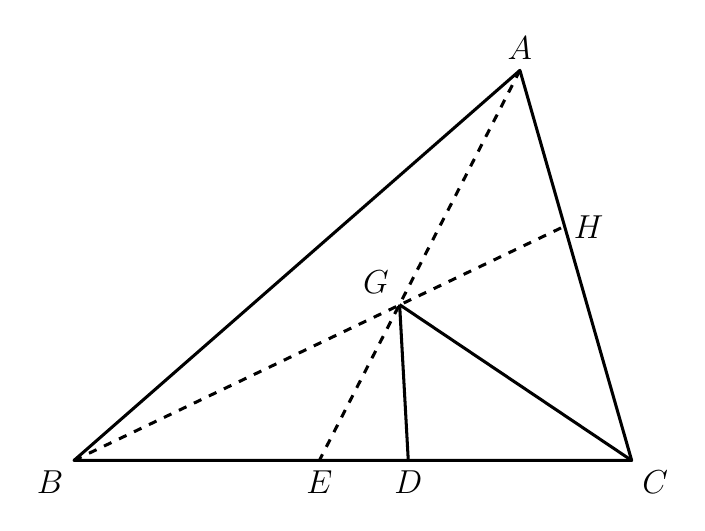
\begin{tikzpicture}[line width=1.1pt, line join=round]
  % Named coordinates (pixels converted with s = 0.009988, centre (457.5, 346))
  \coordinate (A) at (2.122,2.477);
  \coordinate (B) at (-3.541,-2.477);
  \coordinate (C) at (3.541,-2.477);
  \coordinate (D) at (0.704,-2.477);
  \coordinate (E) at (-0.425,-2.477);
  \coordinate (H) at (2.672,0.489);
  \coordinate (G) at (0.594,-0.499);

  % Triangle ABC (solid)
  \draw (A) -- (B) -- (C) -- cycle;

  % Solid segments from C and D to G
  \draw (C) -- (G);
  \draw (D) -- (G);

  % Dashed cevians through G
  \draw[dashed] (A) -- (E);
  \draw[dashed] (B) -- (H);

  % Labels: math italic, enlarged to \large per repair instruction
  \node[above, font=\large] at (A) {$A$};
  \node[below left, font=\large] at (B) {$B$};
  \node[below right, font=\large] at (C) {$C$};
  \node[below, font=\large] at (D) {$D$};
  \node[below, font=\large] at (E) {$E$};
  \node[right, font=\large] at (H) {$H$};
  \node[above left, font=\large] at (G) {$G$};
\end{tikzpicture}
\end{document}